\chapter{Tests und Experimente}
\label{cha:tests}

Im Kapitel Tests und Experimente werden unterschiedliche Hyperparameter-Konfigurationen auf ihre Auswirkungen getestet. Außerdem wird mit unterschiedlichen Netzwerkarchitekturen die Performanz auf Geräten mit leistungsarmer Hardware gemessen.

\section{Auswirkungen der Hyperparameter}

Im Folgenden werden unterschiedliche Kombinationen der Gewichtungsparameter Content-Weight $ \alpha $, Style-Weight $ \beta $ und Total-Variation-Weight $ \gamma $ getestet. Dabei wird als Inhaltsbild  eine eigene Abbildung der HTW-Berlin benutzt. Als Stilbild wird das Kunstwerk \textit{The Starry Night} des Künstlers Vincent Van Gogh und \textit{The Scream} von Edvard Munch verwendet. Die generierten Bilder entsprechen einer Größe von 768 * 768 Pixeln. Die restlichen Hyperparameter werden aus dem Kapitel Methodologie \ref{sec:method_neural_style_transfer} übernommen.

\pagebreak

\subsection{Experiment 1: Starry Night}
\footnotetext[1]{Die Druckversion entspricht nicht der digitalen Qualität der Bilder.}


In diesem Experiment wird das Stilbild \textit{The Starry Night} von Vincent Van Gogh verwendet.

\begin{figure}[H]
    \centering
    \begin{subfigure}[h]{0.32\textwidth}
        \centering
        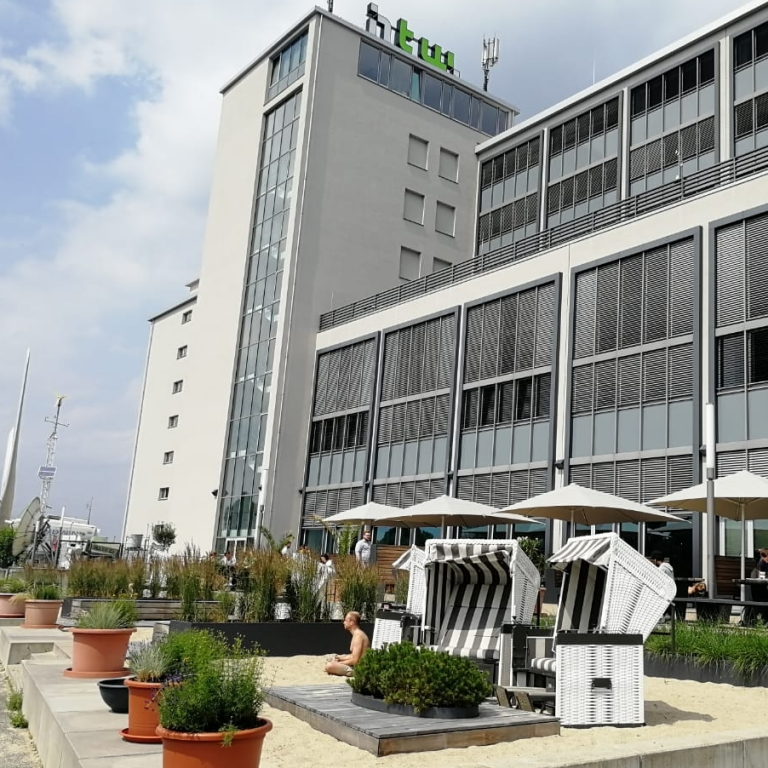
\includegraphics[width=\textwidth]{resources/content/content/htw-768x768.jpg}
    \end{subfigure}
    \begin{subfigure}[h]{0.32\textwidth}
        \centering
        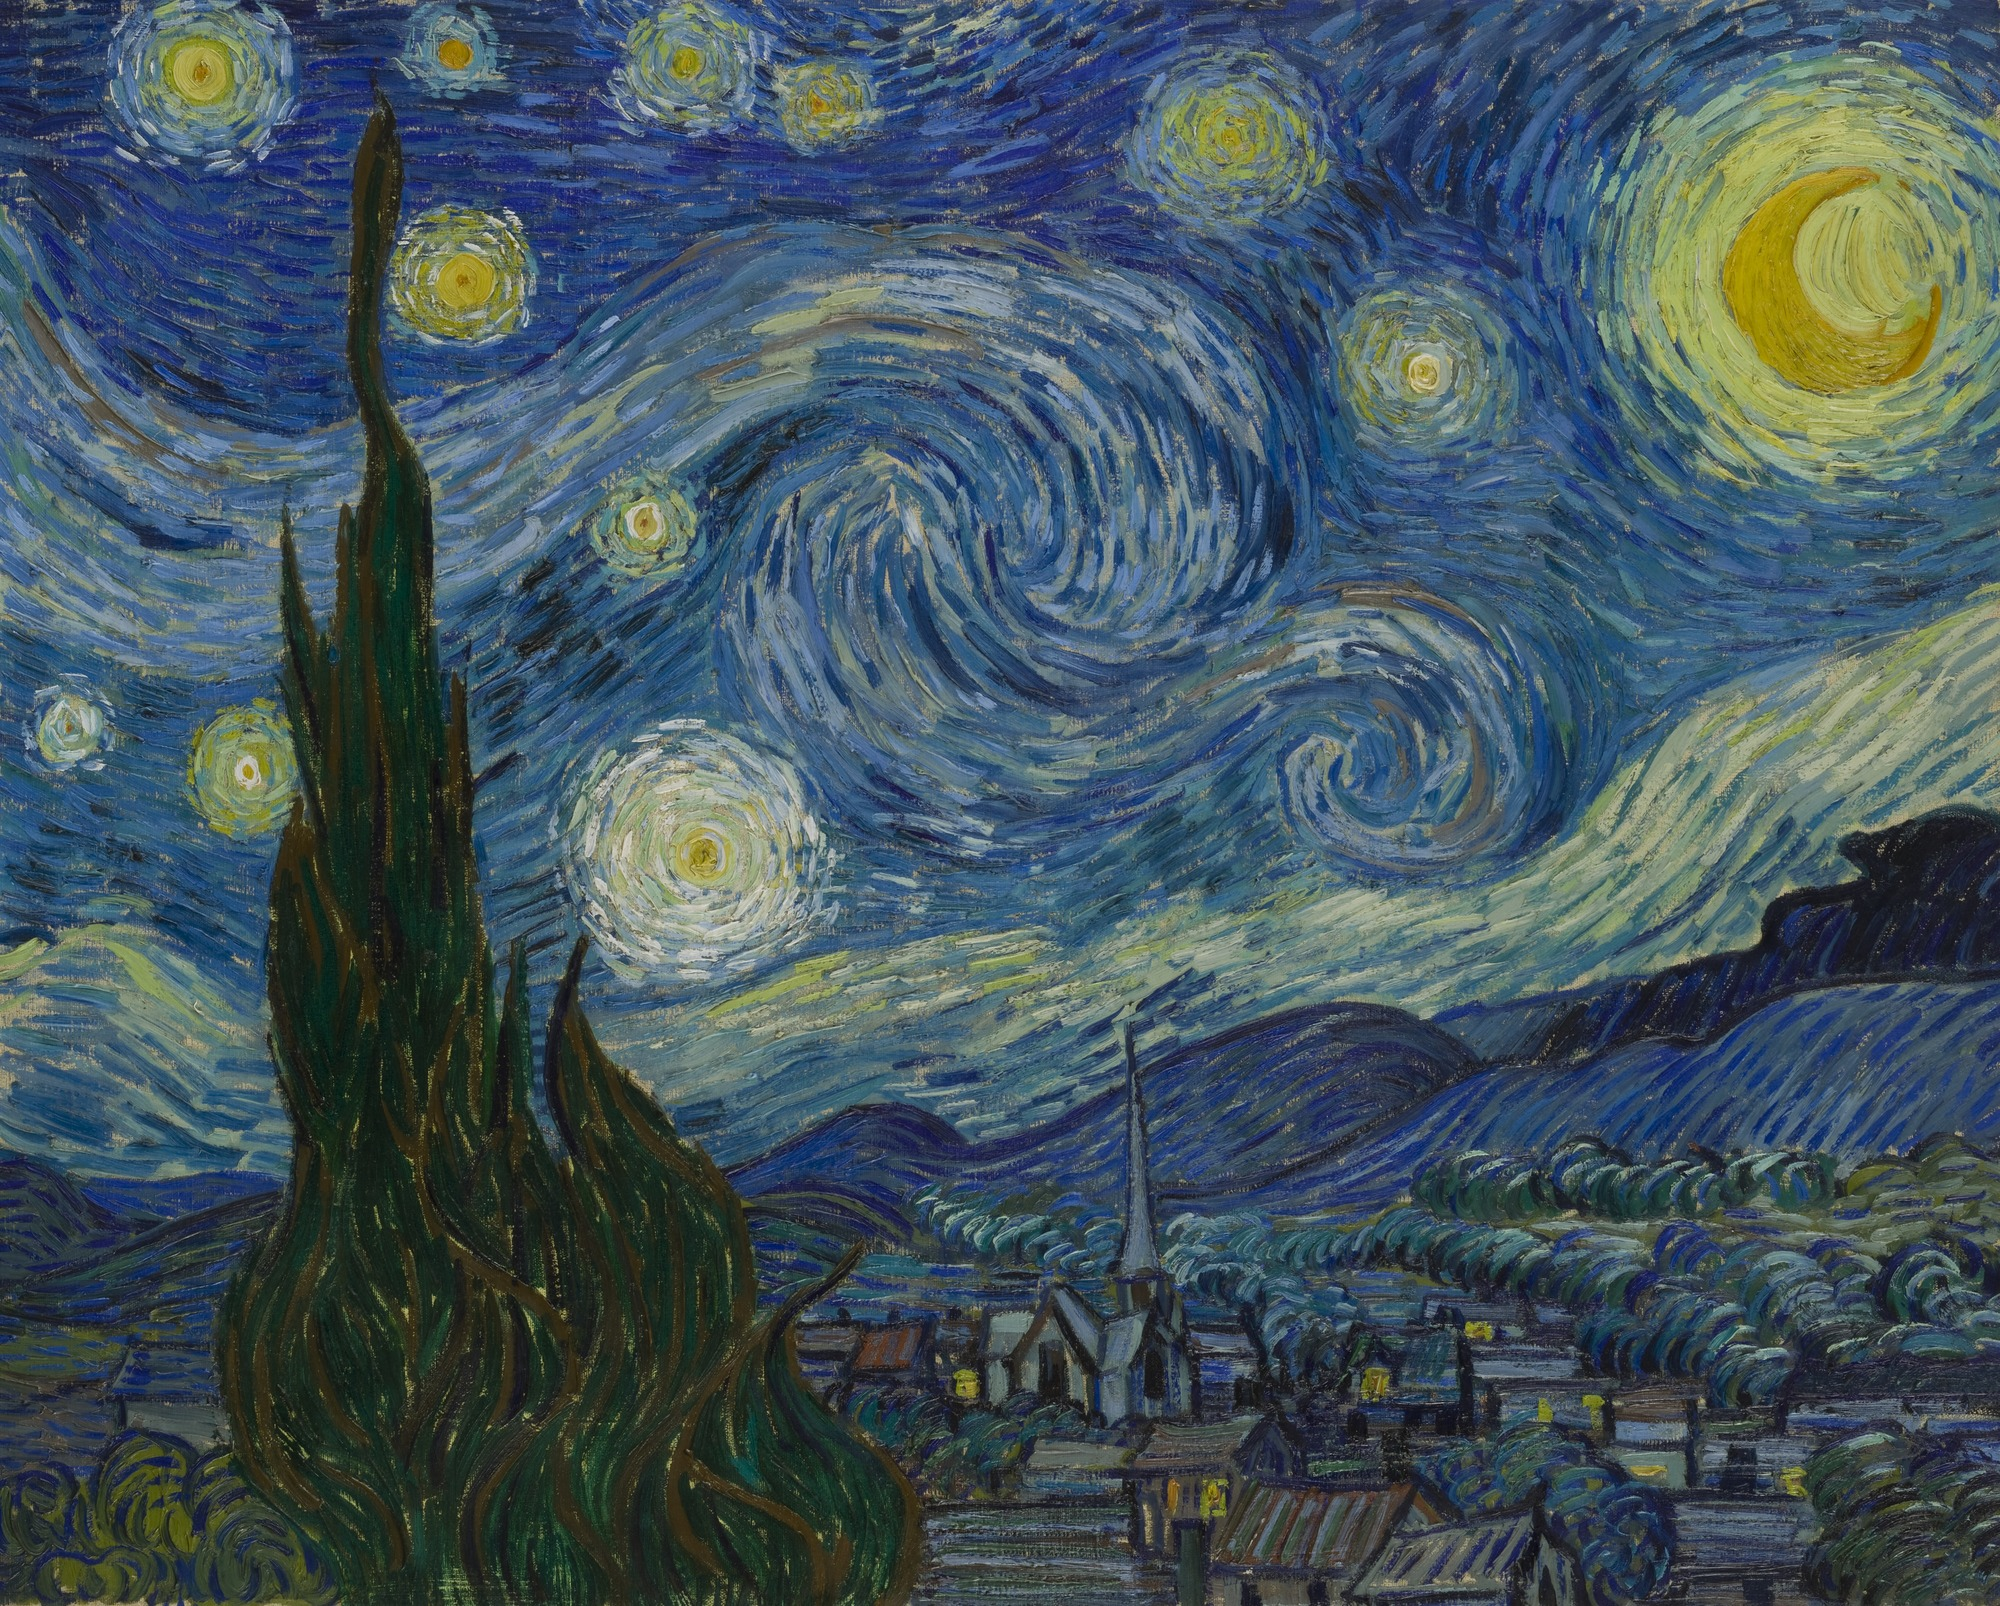
\includegraphics[width=\textwidth]{resources/content/style/the_starry_night.jpg}
    \end{subfigure}
    \caption{HTW kombiniert mit \textit{The Starry Night} \cite{the_starry_night_img}}
\end{figure}

In der ersten Abbildungen werden die verschiedenen
Stilgewichtungen $ \beta = 10^{6} $, $ \beta = 10^{7} $, $ \beta = 10^{8} $ und $ \beta = 10^{9} $ für \textit{The Starry Night} getestet.

\begin{figure}[H]
    \centering
    \begin{subfigure}[h]{0.24\textwidth}
        \centering
        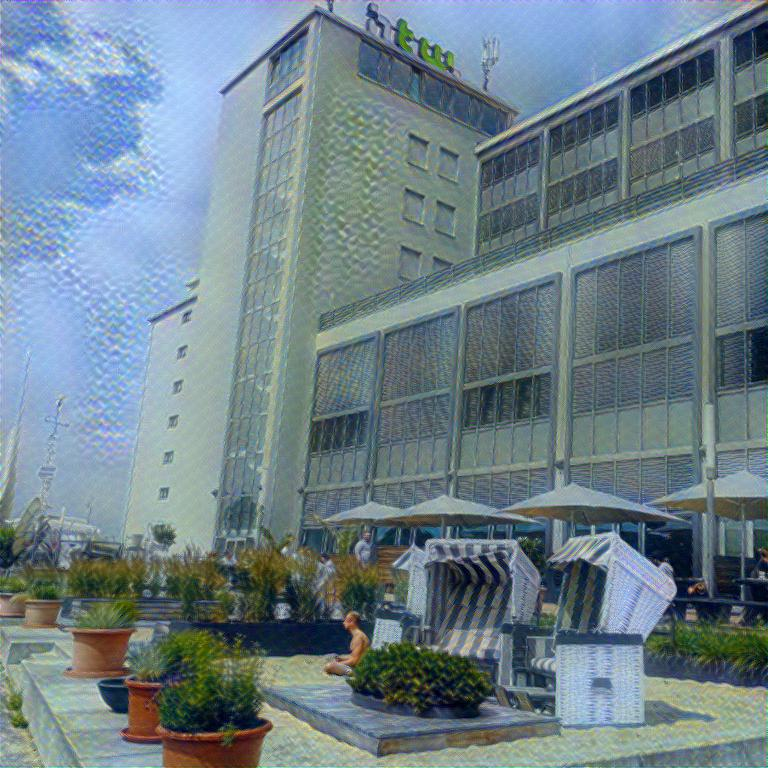
\includegraphics[width=\textwidth]{resources/content/experiments/a__the_starry_night__768x768__style-weight_1e+06__tv-weight_0e+00.jpg}
    \end{subfigure}
    \begin{subfigure}[h]{0.24\textwidth}
        \centering
        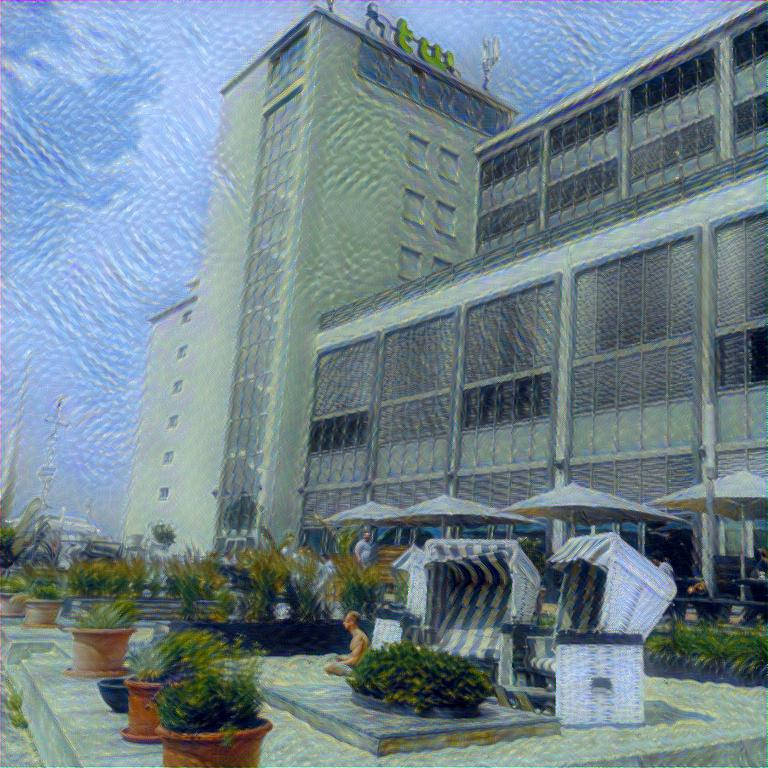
\includegraphics[width=\textwidth]{resources/content/experiments/a__the_starry_night__768x768__style-weight_1e+07__tv-weight_0e+00.jpg}
    \end{subfigure}
    \begin{subfigure}[h]{0.24\textwidth}
        \centering
        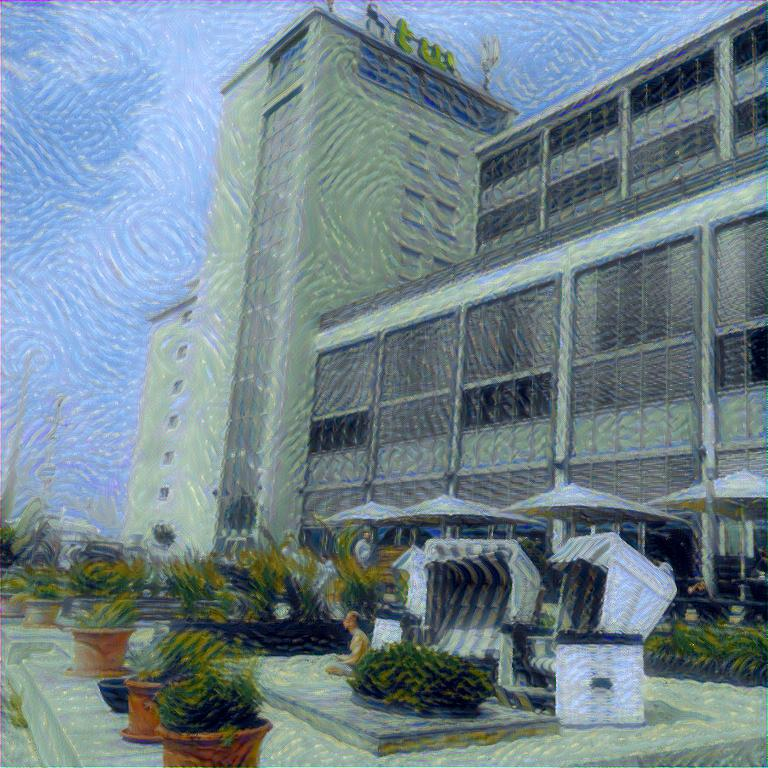
\includegraphics[width=\textwidth]{resources/content/experiments/a__the_starry_night__768x768__style-weight_1e+08__tv-weight_0e+00.jpg}
    \end{subfigure}
    \begin{subfigure}[h]{0.24\textwidth}
        \centering
        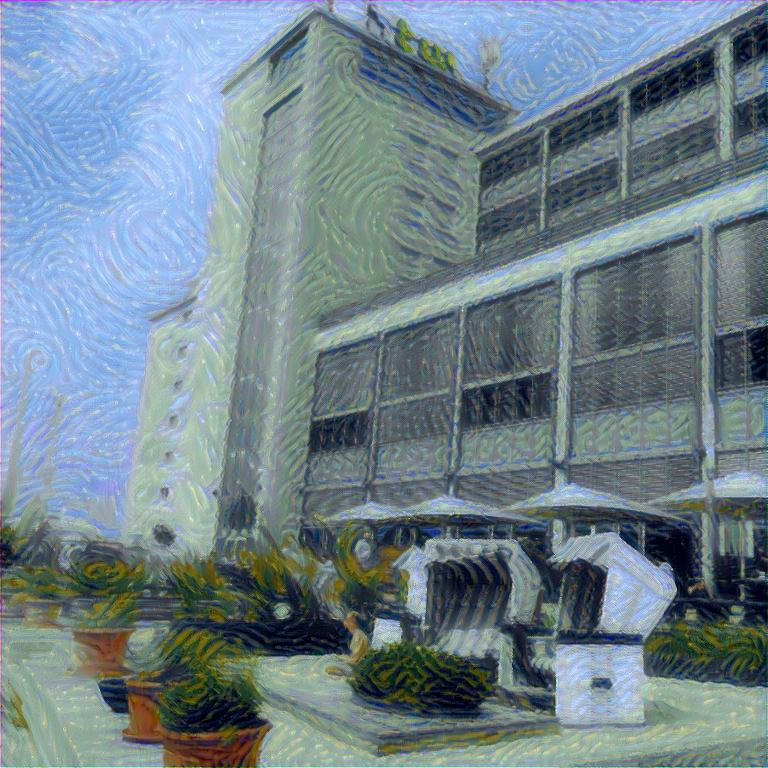
\includegraphics[width=\textwidth]{resources/content/experiments/a__the_starry_night__768x768__style-weight_1e+09__tv-weight_0e+00.jpg}
    \end{subfigure}
    \caption{\textit{The Starry Night} mit $ \alpha = 1 $, $ \beta = 10^{6} - 10^{9} $, $ \gamma = 0 $}
\end{figure}

In der zweiten Abbildungen werden die verschiedenen Total-Variation-Gewichtungen $ \gamma = 10^{-6} $, $ \gamma = 10^{-5} $, $ \gamma = 10^{-4} $ und $ \gamma = 10^{-3} $  für Starry Night getestet.

\begin{figure}[H]
    \centering
    \begin{subfigure}[h]{0.24\textwidth}
        \centering
        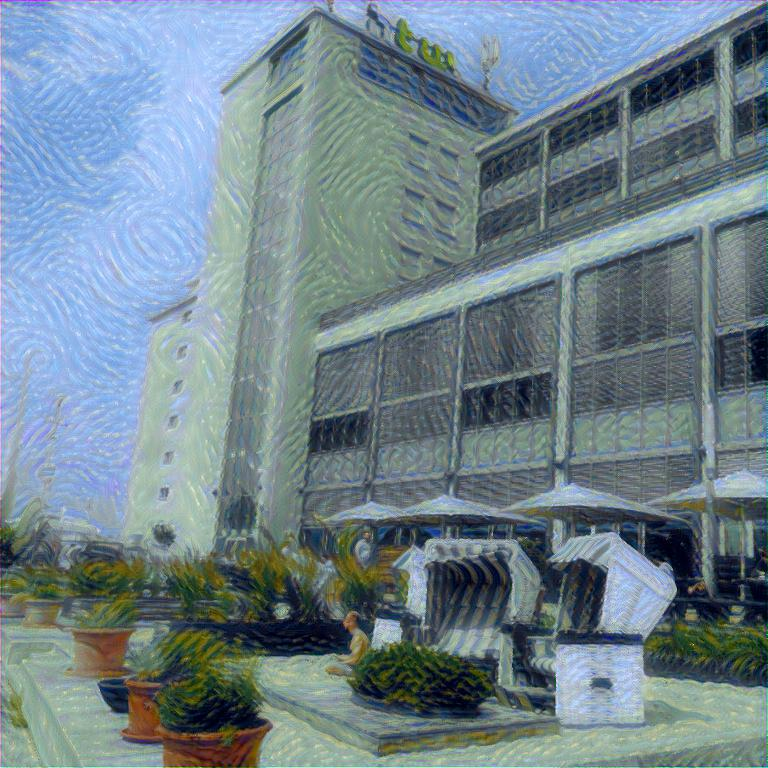
\includegraphics[width=\textwidth]{resources/content/experiments/b__the_starry_night__768x768__style-weight_1e+08__tv-weight_1e-06.jpg}
    \end{subfigure}
    \begin{subfigure}[h]{0.24\textwidth}
        \centering
        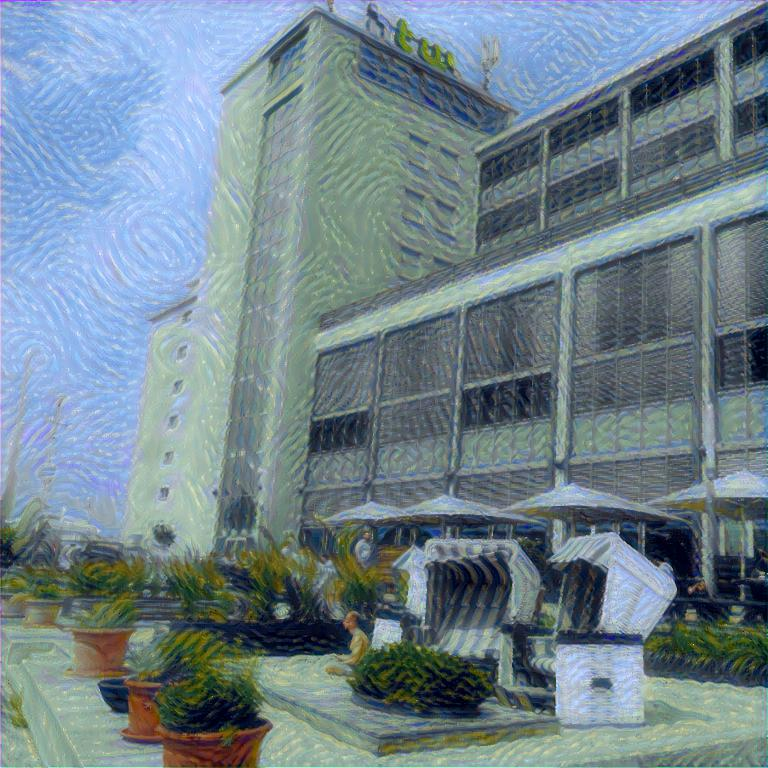
\includegraphics[width=\textwidth]{resources/content/experiments/b__the_starry_night__768x768__style-weight_1e+08__tv-weight_1e-05.jpg}
    \end{subfigure}
    \begin{subfigure}[h]{0.24\textwidth}
        \centering
        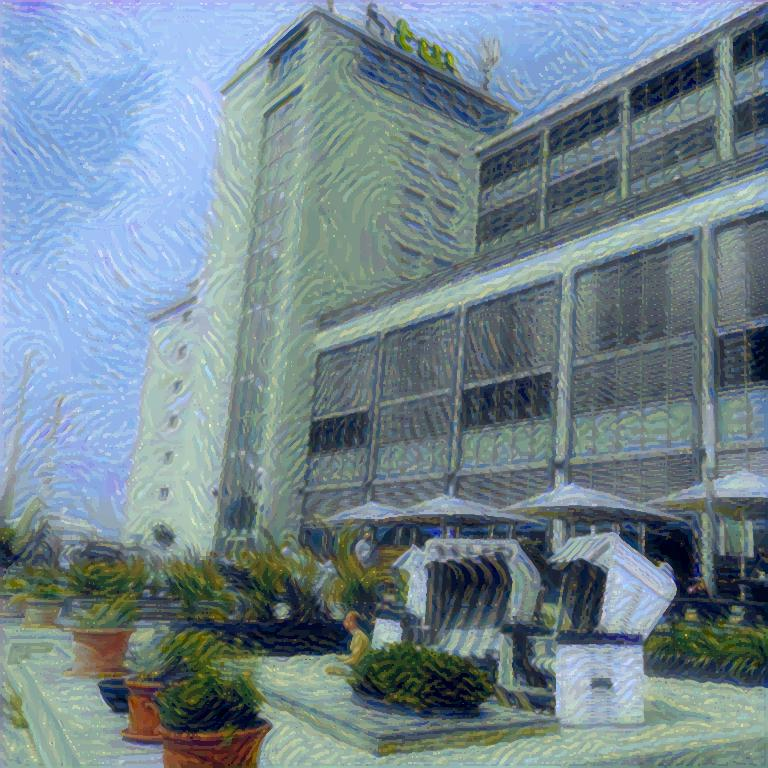
\includegraphics[width=\textwidth]{resources/content/experiments/b__the_starry_night__768x768__style-weight_1e+08__tv-weight_1e-04.jpg}
    \end{subfigure}
    \begin{subfigure}[h]{0.24\textwidth}
        \centering
        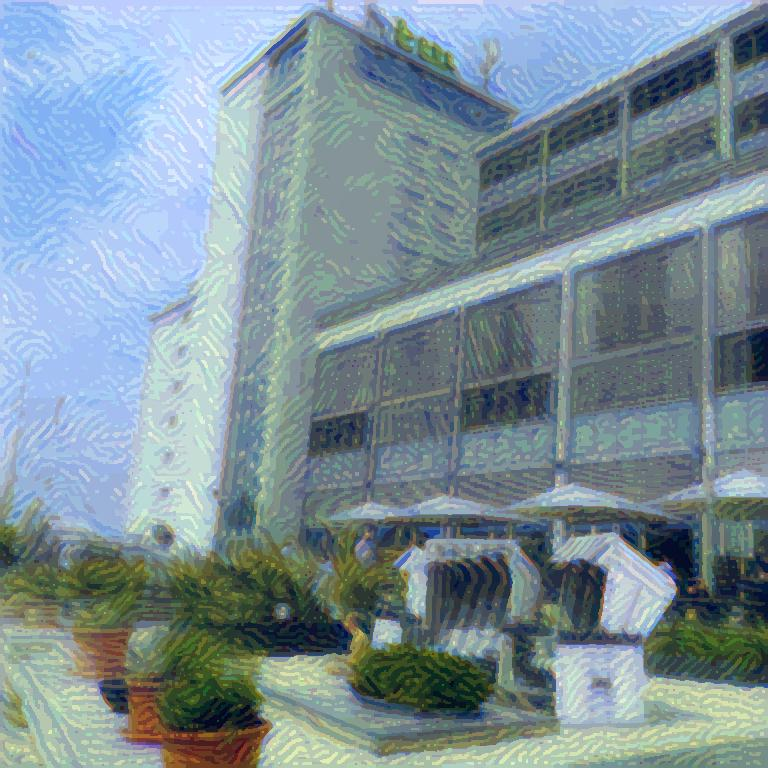
\includegraphics[width=\textwidth]{resources/content/experiments/b__the_starry_night__768x768__style-weight_1e+08__tv-weight_1e-03.jpg}
    \end{subfigure}
    \caption{Starry Night mit $ \alpha = 1 $, $ \beta = 10^{8} $, $ \gamma = 10^{-6} - 10^{-3} $}
\end{figure}

\pagebreak

\subsection{Experiment 2: The Scream}
\footnotetext[1]{Die Druckversion entspricht nicht der digitalen Qualität der Bilder.}

\begin{figure}[H]
    \centering
    \begin{subfigure}[h]{0.32\textwidth}
        \centering
        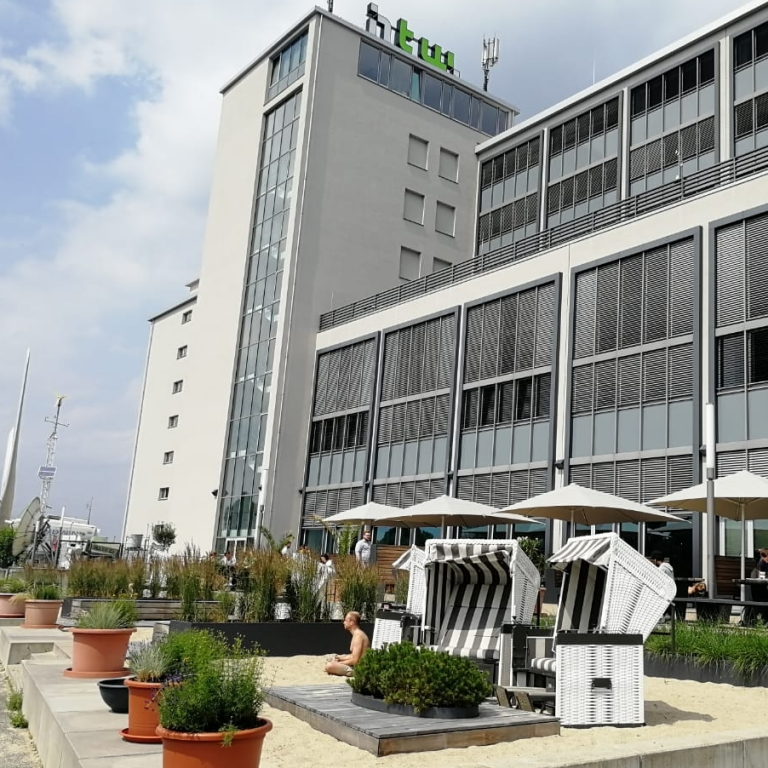
\includegraphics[width=\textwidth]{resources/content/content/htw-768x768.jpg}
    \end{subfigure}
    \begin{subfigure}[h]{0.32\textwidth}
        \centering
        \includegraphics[width=\textwidth]{resources/content/style/the_scream.jpg}
    \end{subfigure}
    \caption{HTW kombiniert mit \textit{The Scream} \cite{the_scream_img}}
\end{figure}

In der ersten Abbildungen werden die verschiedene Stilgewichtungen $ \beta = 10^{6} $, $ \beta = 10^{7} $, $ \beta = 10^{8} $ und $ \beta = 10^{9} $ für \textit{The Scream} getestet.

\begin{figure}[H]
    \centering
    \begin{subfigure}[h]{0.24\textwidth}
        \centering
        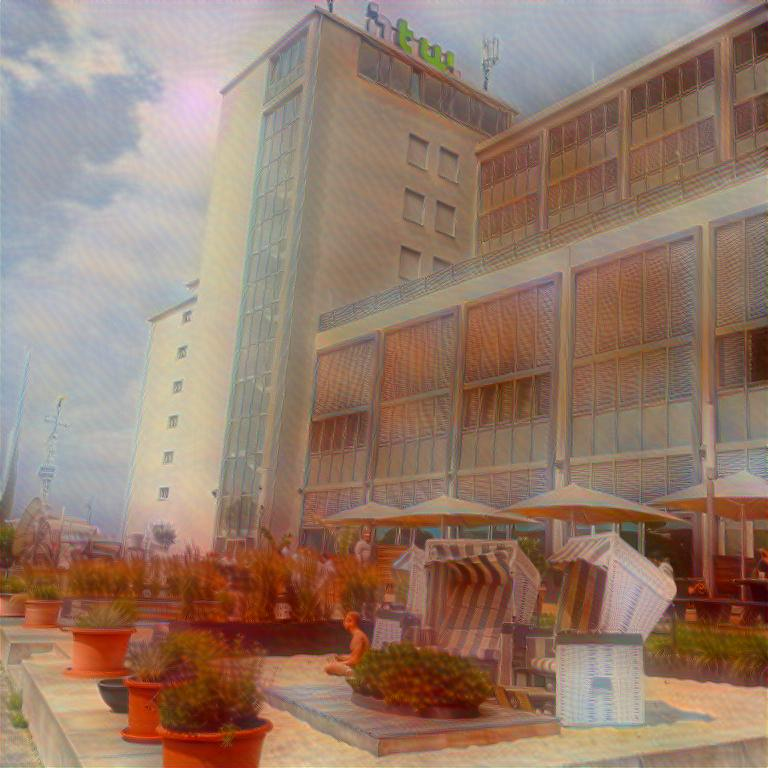
\includegraphics[width=\textwidth]{resources/content/experiments/a__the_scream__768x768__style-weight_1e+06__tv-weight_0e+00.jpg}
    \end{subfigure}
    \begin{subfigure}[h]{0.24\textwidth}
        \centering
        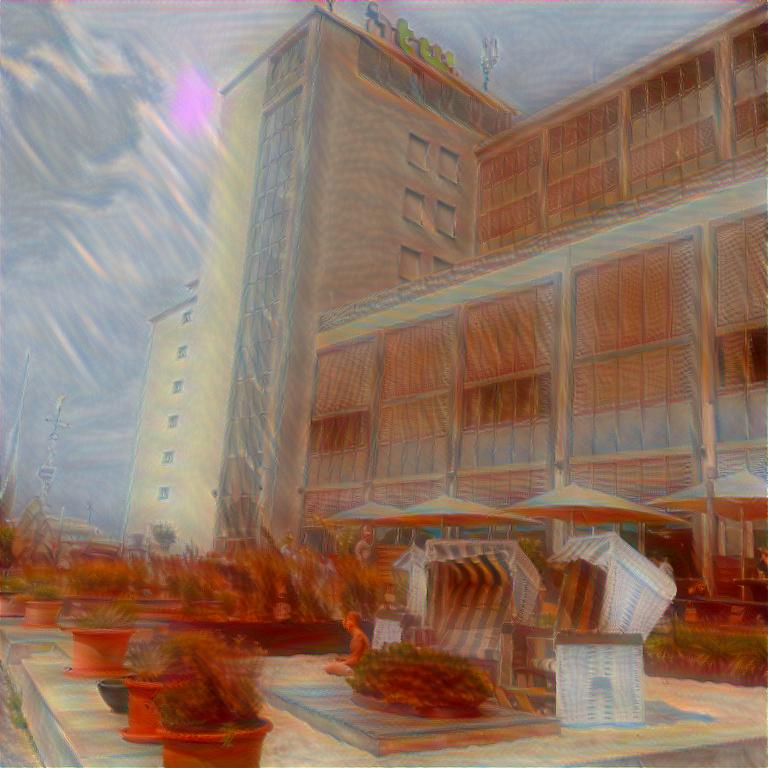
\includegraphics[width=\textwidth]{resources/content/experiments/a__the_scream__768x768__style-weight_1e+07__tv-weight_0e+00.jpg}
    \end{subfigure}
    \begin{subfigure}[h]{0.24\textwidth}
        \centering
        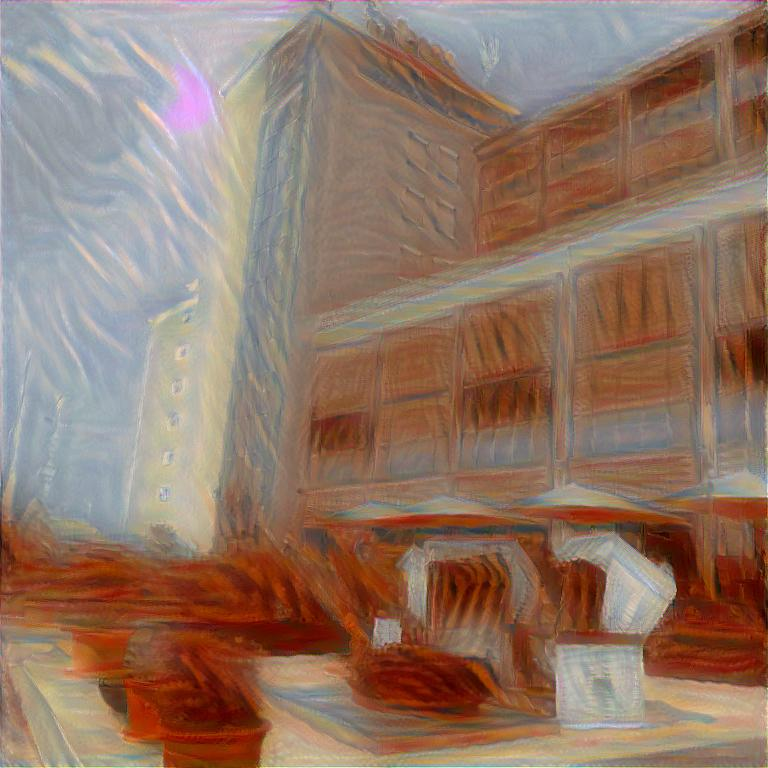
\includegraphics[width=\textwidth]{resources/content/experiments/a__the_scream__768x768__style-weight_1e+08__tv-weight_0e+00.jpg}
    \end{subfigure}
    \begin{subfigure}[h]{0.24\textwidth}
        \centering
        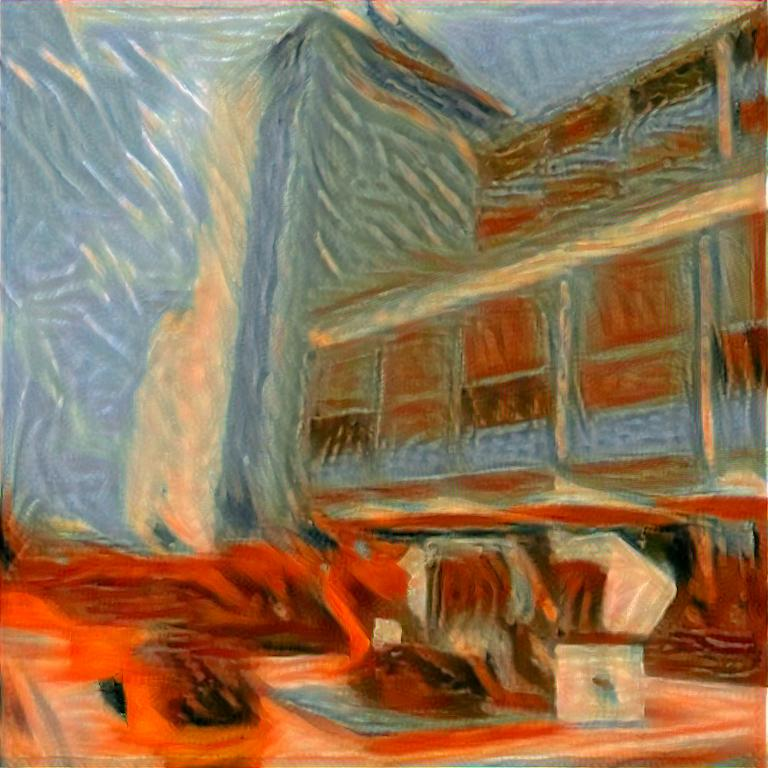
\includegraphics[width=\textwidth]{resources/content/experiments/a__the_scream__768x768__style-weight_1e+09__tv-weight_0e+00.jpg}
    \end{subfigure}
    \caption{\textit{The Scream} mit $ \alpha = 1 $, $ \beta = 10^{6} - 10^{9} $, $ \gamma = 0 $}
\end{figure}

In der zweiten Abbildungen werden die verschiedenen Total-Variation-Gewichtungen $ \gamma = 10^{-6} $, $ \gamma = 10^{-5} $, $ \gamma = 10^{-4} $ und $ \gamma = 10^{-3} $ für \textit{The Scream} getestet.

\begin{figure}[H]
    \centering
    \begin{subfigure}[h]{0.24\textwidth}
        \centering
        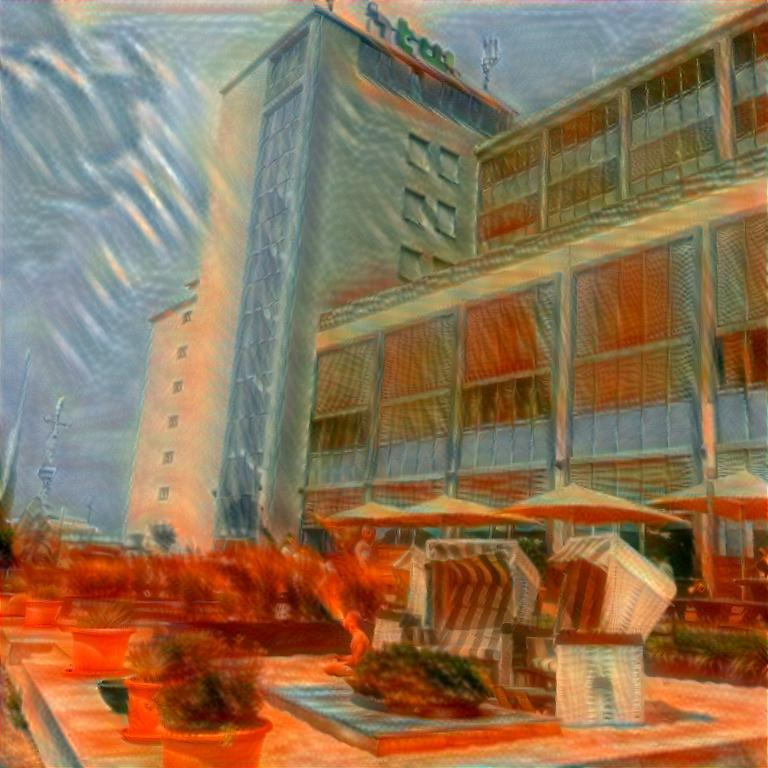
\includegraphics[width=\textwidth]{resources/content/experiments/b__the_scream__768x768__style-weight_1e+07__tv-weight_1e-06.jpg}
    \end{subfigure}
    \begin{subfigure}[h]{0.24\textwidth}
        \centering
        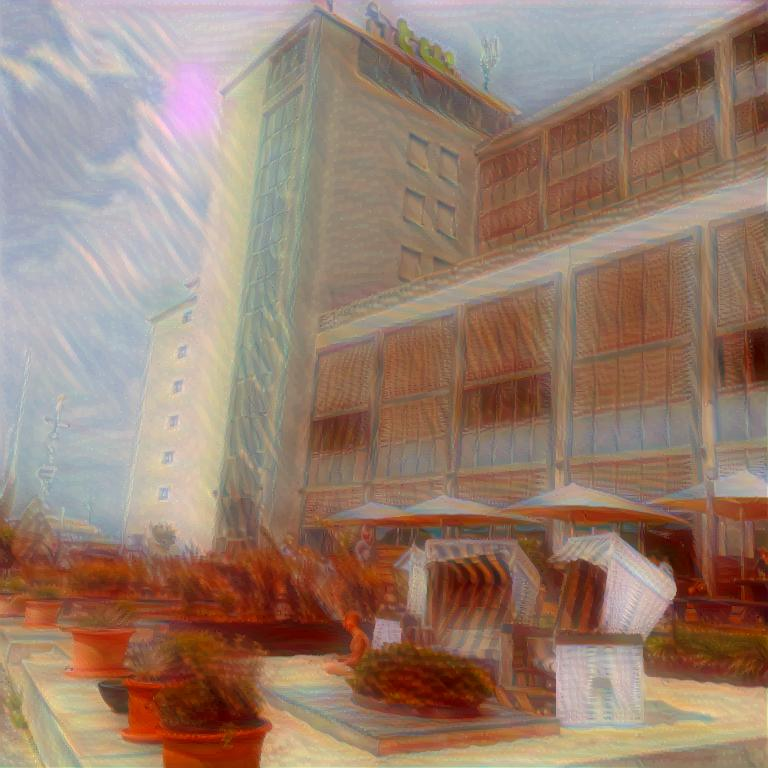
\includegraphics[width=\textwidth]{resources/content/experiments/b__the_scream__768x768__style-weight_1e+07__tv-weight_1e-05.jpg}
    \end{subfigure}
    \begin{subfigure}[h]{0.24\textwidth}
        \centering
        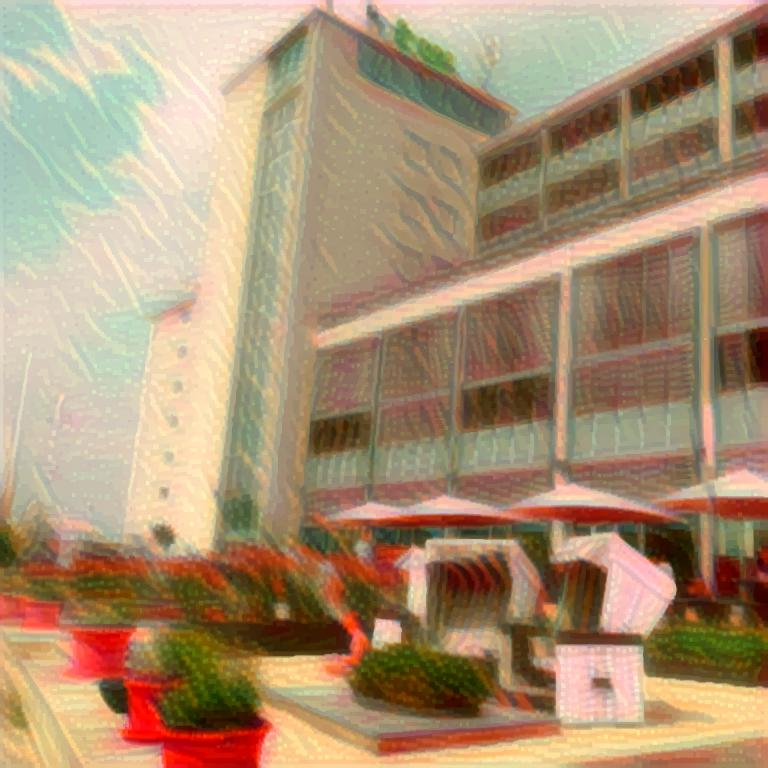
\includegraphics[width=\textwidth]{resources/content/experiments/b__the_scream__768x768__style-weight_1e+07__tv-weight_1e-04.jpg}
    \end{subfigure}
    \begin{subfigure}[h]{0.24\textwidth}
        \centering
        
\includegraphics[width=\textwidth]{resources/content/experiments/b__the_scream__768x768__style-weight_1e+07__tv-weight_1e-03.jpg}
    \end{subfigure}
    \caption{\textit{The Scream} mit $ \alpha = 1 $, $ \beta = 10^{7} $, $ \gamma = 10^{-6} - 10^{-3} $}
\end{figure}

\pagebreak

\subsection{Interpretation der Ergebnisse}

Wie bei beiden Tests zu sehen ist, werden die Muster mit zunehmendem Style-Weight $ \beta $ auf dem Ausgangsbild immer stärker generiert. Mit $ b = 10^{5} $ sind bei beiden Stilen die Muster des Gemäldes kaum noch zu erkennen. Lediglich wird das Ausgangsbild den Farben des Stilbildes angepasst. Ein optisch ansprechender Effekt ergibt sich bei beiden Stilen ab $ \beta = 10^{7} $. 

Mit zunehmendem Total-Variation-Weight $ \gamma $ fließen die Farben mehr ineinander und das Ausgangsbild wird verschwommener. Das ist besonders gut zu sehen bei \textit{The Starry Night} mit $ \gamma = 10^{-3} $ und \text{\textit{The Scream}} mit $ \gamma = 10^{-4} $.


\section{Auswirkungen der Netzwerkarchitekturen}

In diesem Experiment wurden drei unterschiedliche Bildgrößen auf verschiedenen Geräten auf Durchführbarkeit und Performanz getestet.
Gemessen wird die Berechnungsgeschwindigkeit beim Forward-Pass durch das Netzwerk. Ein bereits erster Indikator für die Performanz eines Neuronalen Netzwerks ist die Anzahl der lernbaren Parameter, die bei der Trainingsphase optimiert werden. Erstellt wurden 16 unterschiedliche Netzwerke mit verschiedenen Kombinationen für $ m $ und $ s $, vgl. \ref{tab:networks}. 

\subsection{Verwendete Geräte}

Bei der Berechnung des Forward-Pass macht es einen Unterschied, ob sie auf dem CPU oder dem GPU eines Geräts durchgeführt wird. Neuronale Netzwerke können auf einer GPU schneller als auf einem CPU berechnet werden. Das liegt daran, dass eine GPU besonders auf die Berechnung von Matrix-Operationen (wie Sie auch bei grafischen Anwendungen benutzt werden) spezialisiert ist.

Die Daten werden beim Einsatz des GPUs in den Grafikspeicher geladen. Bei der Berechnung über den CPU wird der Arbeitsspeicher (RAM) des Geräts verwendet.

\pagebreak

\subsubsection{Gerät 1: Dell XPS 15 9550}

Beim Dell XPS 15 9550 handelt es sich um einen handelsüblichen Laptop aus dem Jahr 2016.

\begin{table}[H]
    \centering
    \begin{tabular}{ |c|c| }
        \hline
        Prozessor       & Intel Core i7-6700HQ \\ \hline
        Grafikkarte     & NVIDIA® GeForce™ GTX 960M (2GB GDDR5) \\ \hline
        Arbeitsspeicher & 16GB DDR4  \\ \hline
        Festplatte      & 512GB SSD \\ \hline
    \end{tabular}
    \caption{Spezifikation: Dell XPS 15 9550}
    \label{tab:xps15}
\end{table}

\subsubsection{Gerät 2: Jetson TX2}

Beim Jetson TX2 handelt es sich um ein leistungsarmes Gerät für die Realiserung von Algorithmen der künstlichen Intelligenz auf eingebetteten Systemen.

\begin{table}[H]
    \centering
    \begin{tabular}{ |c|c| }
        \hline
        Prozessor       & Dual-Core NVIDIA Denver 2 64-Bit CPU, Quad-Core ARM®Cortex®-A57 MPCore \\ \hline
        Grafikkarte     & 256-core NVIDIA Maxwell™ GPU \\ \hline
        Arbeitsspeicher & 8GB 128-bit LPDDR4 Memory  \\ \hline
        Festplatte      & 32GB eMMC 5.1 \\ \hline
    \end{tabular}
    \caption{Spezifikation: Jetson TX2}
    \label{tab:jetson_tx1}
\end{table}

\subsection{Durchführung der Experimente}

Alle Netzwerke wurden mit einer Batch-Size von $ 24 $, Bildgrößen von 224 * 224 Pixeln und einer Learning-Rate von $ 10^{-3} $ trainiert. Es wurden 6 Epochen der Trainingsdaten aus dem Jahr 2017 des COCO-Datensatzes verwendet, welche $ 118287 $ Bilder enthalten. Insgesamt wurden die Modelle mit $ 709722 $ Bildern trainiert. Dabei lag die Trainingszeit auf einem Server mit einem GeForce GTX 1080 Ti GPU pro Modell zwischen 5 und 10 Stunden.

Beim Training fiel auf, dass die generierten Bilder großflächige, schwarze oder weiße Artefakte enthielten. Ein Austausch der finalen Aktivierungsfunktion HardTanH, vgl. \ref{sec:hardtanh}, mit der Sigmoid-Aktivierungsfunktion, vgl. \ref{sec:sigmoid}, konnte das Problem lösen.

Abschließend wurden die unterschiedlichen Netzwerkarchitekturen auf ihre Performanz getestet. Tests, die wegen unzureichendem Arbeitsspeicher oder Grafikspeicher fehlschlugen, wurden als \textcolor{danger}{nicht durchführbar} gekennzeichnet. Um die Tests durchzuführen, wurden Bilder der Größen 1920 * 1080 Pixel, 1024 * 786 Pixel und 640 * 480 Pixel jeweils 10 mal mit jedem Netzwerk berechnet, die Berechnugnsgeschwindigkeit gemessen, und das arithmische Mittel der 10 Durchläufe gebildet. Die Ergebnisse sind in den Anlagen \ref{tab:1920x1080}, \ref{tab:1024x768} und \ref{tab:640x480} angefügt.

\subsection{Interpretation der Ergebnisse}

Die Performanz-Tests haben ergeben, dass der Jetson TX2 mit fast allen Netzwerkarchitekturen in der Lage war, den Style-Transfer durchzuführen. Für Bilder der Größe 1920 * 768 Pixel war es jedoch nicht möglich, Netzwerk 1 und Netzwerk 5 zu verwenden, vlg. \ref{tab:1920x1080}. Alle anderen Netzwerkarchitekturen konnten für Full HD Bilder in weniger als einer Sekunde berechnet werden.

Die Abbildungen \ref{img:loss_the_starry_night} und \ref{img:loss_the_scream} stellen die Loss-Kurven beim Trainingsverlauf aller Netzwerke dar. Die Loss-Kurven wurden dabei mit einem laufenden arithmetischen Mittel über 100 Iterationen geflächt, um die Ergebnisse besser darstellen zu können. Für beide Stilbilder ergibt sich ein ähnlicher Trainingsverlauf. Die Netzwerkarchitekturen mit mehr lernbaren Parametern erreichen ein niedrigeres Endloss. Eine Ausnahme bilden dabei die Netzwerke mit dem Parameter $ m = 16 $. Sie erreichen in allen Fällen das niedrigste Endloss. In den Abbildungen sind die Loss-Kurven dieser Netzwerke mit einer stärkeren Linie gekennzeichnet.

Desweiteren wurden die optischen Ergebnisse aller Netzwerkarchitekturen getestet. Die Ergebnisse sind in \ref{img:results_the_starry_night} und \ref{img:results_the_scream} dargestellt. Wieder zeigt sich, dass Netzwerke mit dem Parameter $ m = 16 $ optisch vielfältigere Bilder generieren als die anderen Netzwerke. Daraus wird geschlussfolgert, dass die optische Vielfalt der generierten Bilder mit dem Loss zusammenhängt.

\subsection{Weitere Ergebnisse}

Auf Basis der zuvor gewonnen Erkenntniss wurden weitere Modelle mit unterschiedlichen Stilbildern trainiert. Für das Training wurde jeweils die Netzwerkarchitektur 2, $ m = 16 $ und $ s = 5 $, verwendet, die in den durchgeführten Tests am besten abschnitt. Die Abbildungen \ref{img:trained_models1}, \ref{img:trained_models2} und \ref{img:trained_models3} zeigen Beispiele erfolgreich trainierter Stilmodelle.